\documentclass[12pt]{article}

%packages
%\usepackage{latexsym}
\usepackage{graphicx}
\usepackage{color}
\usepackage{amsmath}
\usepackage{dsfont}
\usepackage{placeins}
\usepackage{amssymb}
\usepackage{wasysym}
\usepackage{abstract}
\usepackage{hyperref}
\usepackage{etoolbox}
\usepackage{datetime}
\usepackage{xcolor}
\usepackage{alphalph}
\usepackage{accents}

\settimeformat{ampmtime}

%\usepackage{pstricks,pst-node,pst-tree}

%\usepackage{algpseudocode}
%\usepackage{amsthm}
%\usepackage{hyperref}
%\usepackage{mathrsfs}
%\usepackage{amsfonts}
%\usepackage{bbding}
%\usepackage{listings}
%\usepackage{appendix}
\usepackage[margin=1in]{geometry}
%\geometry{papersize={8.5in,11in},total={6.5in,9in}}
%\usepackage{cancel}
%\usepackage{algorithmic, algorithm}

\makeatletter
\def\maxwidth{ %
  \ifdim\Gin@nat@width>\linewidth
    \linewidth
  \else
    \Gin@nat@width
  \fi
}
\makeatother

\definecolor{fgcolor}{rgb}{0.345, 0.345, 0.345}
\newcommand{\hlnum}[1]{\textcolor[rgb]{0.686,0.059,0.569}{#1}}%
\newcommand{\hlstr}[1]{\textcolor[rgb]{0.192,0.494,0.8}{#1}}%
\newcommand{\hlcom}[1]{\textcolor[rgb]{0.678,0.584,0.686}{\textit{#1}}}%
\newcommand{\hlopt}[1]{\textcolor[rgb]{0,0,0}{#1}}%
\newcommand{\hlstd}[1]{\textcolor[rgb]{0.345,0.345,0.345}{#1}}%
\newcommand{\hlkwa}[1]{\textcolor[rgb]{0.161,0.373,0.58}{\textbf{#1}}}%
\newcommand{\hlkwb}[1]{\textcolor[rgb]{0.69,0.353,0.396}{#1}}%
\newcommand{\hlkwc}[1]{\textcolor[rgb]{0.333,0.667,0.333}{#1}}%
\newcommand{\hlkwd}[1]{\textcolor[rgb]{0.737,0.353,0.396}{\textbf{#1}}}%

\usepackage{framed}
\makeatletter
\newenvironment{kframe}{%
 \def\at@end@of@kframe{}%
 \ifinner\ifhmode%
  \def\at@end@of@kframe{\end{minipage}}%
  \begin{minipage}{\columnwidth}%
 \fi\fi%
 \def\FrameCommand##1{\hskip\@totalleftmargin \hskip-\fboxsep
 \colorbox{shadecolor}{##1}\hskip-\fboxsep
     % There is no \\@totalrightmargin, so:
     \hskip-\linewidth \hskip-\@totalleftmargin \hskip\columnwidth}%
 \MakeFramed {\advance\hsize-\width
   \@totalleftmargin\z@ \linewidth\hsize
   \@setminipage}}%
 {\par\unskip\endMakeFramed%
 \at@end@of@kframe}
\makeatother

\definecolor{shadecolor}{rgb}{.77, .77, .77}
\definecolor{messagecolor}{rgb}{0, 0, 0}
\definecolor{warningcolor}{rgb}{1, 0, 1}
\definecolor{errorcolor}{rgb}{1, 0, 0}
\newenvironment{knitrout}{}{} % an empty environment to be redefined in TeX

\usepackage{alltt}
\usepackage[T1]{fontenc}

\newcommand{\qu}[1]{``#1''}
\newcounter{probnum}
\setcounter{probnum}{1}

%create definition to allow local margin changes
\def\changemargin#1#2{\list{}{\rightmargin#2\leftmargin#1}\item[]}
\let\endchangemargin=\endlist 

%allow equations to span multiple pages
\allowdisplaybreaks

%define colors and color typesetting conveniences
\definecolor{gray}{rgb}{0.5,0.5,0.5}
\definecolor{black}{rgb}{0,0,0}
\definecolor{white}{rgb}{1,1,1}
\definecolor{blue}{rgb}{0.5,0.5,1}
\newcommand{\inblue}[1]{\color{blue}#1 \color{black}}
\definecolor{green}{rgb}{0.133,0.545,0.133}
\newcommand{\ingreen}[1]{\color{green}#1 \color{black}}
\definecolor{yellow}{rgb}{1,1,0}
\newcommand{\inyellow}[1]{\color{yellow}#1 \color{black}}
\definecolor{orange}{rgb}{0.9,0.649,0}
\newcommand{\inorange}[1]{\color{orange}#1 \color{black}}
\definecolor{red}{rgb}{1,0.133,0.133}
\newcommand{\inred}[1]{\color{red}#1 \color{black}}
\definecolor{purple}{rgb}{0.58,0,0.827}
\newcommand{\inpurple}[1]{\color{purple}#1 \color{black}}
\definecolor{backgcode}{rgb}{0.97,0.97,0.8}
\definecolor{Brown}{cmyk}{0,0.81,1,0.60}
\definecolor{OliveGreen}{cmyk}{0.64,0,0.95,0.40}
\definecolor{CadetBlue}{cmyk}{0.62,0.57,0.23,0}

%define new math operators
\DeclareMathOperator*{\argmax}{arg\,max~}
\DeclareMathOperator*{\argmin}{arg\,min~}
\DeclareMathOperator*{\argsup}{arg\,sup~}
\DeclareMathOperator*{\arginf}{arg\,inf~}
\DeclareMathOperator*{\convolution}{\text{\Huge{$\ast$}}}
\newcommand{\infconv}[2]{\convolution^\infty_{#1 = 1} #2}
%true functions

%%%% GENERAL SHORTCUTS

%shortcuts for pure typesetting conveniences
\newcommand{\bv}[1]{\boldsymbol{#1}}

%shortcuts for compound constants
\newcommand{\BetaDistrConst}{\dfrac{\Gamma(\alpha + \beta)}{\Gamma(\alpha)\Gamma(\beta)}}
\newcommand{\NormDistrConst}{\dfrac{1}{\sqrt{2\pi\sigma^2}}}

%shortcuts for conventional symbols
\newcommand{\tsq}{\tau^2}
\newcommand{\tsqh}{\hat{\tau}^2}
\newcommand{\sigsq}{\sigma^2}
\newcommand{\sigsqsq}{\parens{\sigma^2}^2}
\newcommand{\sigsqovern}{\dfrac{\sigsq}{n}}
\newcommand{\tausq}{\tau^2}
\newcommand{\tausqalpha}{\tau^2_\alpha}
\newcommand{\tausqbeta}{\tau^2_\beta}
\newcommand{\tausqsigma}{\tau^2_\sigma}
\newcommand{\betasq}{\beta^2}
\newcommand{\sigsqvec}{\bv{\sigma}^2}
\newcommand{\sigsqhat}{\hat{\sigma}^2}
\newcommand{\sigsqhatmlebayes}{\sigsqhat_{\text{Bayes, MLE}}}
\newcommand{\sigsqhatmle}[1]{\sigsqhat_{#1, \text{MLE}}}
\newcommand{\bSigma}{\bv{\Sigma}}
\newcommand{\bSigmainv}{\bSigma^{-1}}
\newcommand{\thetavec}{\bv{\theta}}
\newcommand{\thetahat}{\hat{\theta}}
\newcommand{\thetahatmle}{\hat{\theta}_{\mathrm{MLE}}}
\newcommand{\thetavechatmle}{\hat{\thetavec}_{\mathrm{MLE}}}
\newcommand{\muhat}{\hat{\mu}}
\newcommand{\musq}{\mu^2}
\newcommand{\muvec}{\bv{\mu}}
\newcommand{\muhatmle}{\muhat_{\text{MLE}}}
\newcommand{\lambdahat}{\hat{\lambda}}
\newcommand{\lambdahatmle}{\lambdahat_{\text{MLE}}}
\newcommand{\etavec}{\bv{\eta}}
\newcommand{\alphavec}{\bv{\alpha}}
\newcommand{\minimaxdec}{\delta^*_{\mathrm{mm}}}
\newcommand{\ybar}{\bar{y}}
\newcommand{\xbar}{\bar{x}}
\newcommand{\Xbar}{\bar{X}}
\newcommand{\phat}{\hat{p}}
\newcommand{\Phat}{\hat{P}}
\newcommand{\Zbar}{\bar{Z}}
\newcommand{\iid}{~{\buildrel iid \over \sim}~}
\newcommand{\inddist}{~{\buildrel ind \over \sim}~}
\newcommand{\approxdist}{~{\buildrel approx \over \sim}~}
\newcommand{\equalsindist}{~{\buildrel d \over =}~}
\newcommand{\loglik}[1]{\ell\parens{#1}}
\newcommand{\thetahatkminone}{\thetahat^{(k-1)}}
\newcommand{\thetahatkplusone}{\thetahat^{(k+1)}}
\newcommand{\thetahatk}{\thetahat^{(k)}}
\newcommand{\half}{\frac{1}{2}}
\newcommand{\third}{\frac{1}{3}}
\newcommand{\twothirds}{\frac{2}{3}}
\newcommand{\fourth}{\frac{1}{4}}
\newcommand{\fifth}{\frac{1}{5}}
\newcommand{\sixth}{\frac{1}{6}}

%shortcuts for vector and matrix notation
\newcommand{\A}{\bv{A}}
\newcommand{\At}{\A^T}
\newcommand{\Ainv}{\inverse{\A}}
\newcommand{\B}{\bv{B}}
\newcommand{\K}{\bv{K}}
\newcommand{\Kt}{\K^T}
\newcommand{\Kinv}{\inverse{K}}
\newcommand{\Kinvt}{(\Kinv)^T}
\newcommand{\M}{\bv{M}}
\newcommand{\Bt}{\B^T}
\newcommand{\Q}{\bv{Q}}
\newcommand{\Qt}{\Q^T}
\newcommand{\R}{\bv{R}}
\newcommand{\Rt}{\R^T}
\newcommand{\Z}{\bv{Z}}
\newcommand{\X}{\bv{X}}
\newcommand{\Xsub}{\X_{\text{(sub)}}}
\newcommand{\Xsubadj}{\X_{\text{(sub,adj)}}}
\newcommand{\I}{\bv{I}}
\newcommand{\Y}{\bv{Y}}
\newcommand{\sigsqI}{\sigsq\I}
\renewcommand{\P}{\bv{P}}
\newcommand{\Psub}{\P_{\text{(sub)}}}
\newcommand{\Pt}{\P^T}
\newcommand{\Pii}{P_{ii}}
\newcommand{\Pij}{P_{ij}}
\newcommand{\IminP}{(\I-\P)}
\newcommand{\Xt}{\bv{X}^T}
\newcommand{\XtX}{\Xt\X}
\newcommand{\XtXinv}{\parens{\Xt\X}^{-1}}
\newcommand{\XtXinvXt}{\XtXinv\Xt}
\newcommand{\XXtXinvXt}{\X\XtXinvXt}
\newcommand{\x}{\bv{x}}
\newcommand{\onevec}{\bv{1}}
\newcommand{\oneton}{1, \ldots, n}
\newcommand{\yoneton}{y_1, \ldots, y_n}
\newcommand{\yonetonorder}{y_{(1)}, \ldots, y_{(n)}}
\newcommand{\Yoneton}{Y_1, \ldots, Y_n}
\newcommand{\iinoneton}{i \in \braces{\oneton}}
\newcommand{\onetom}{1, \ldots, m}
\newcommand{\jinonetom}{j \in \braces{\onetom}}
\newcommand{\xoneton}{x_1, \ldots, x_n}
\newcommand{\Xoneton}{X_1, \ldots, X_n}
\newcommand{\xt}{\x^T}
\newcommand{\y}{\bv{y}}
\newcommand{\yt}{\y^T}
\renewcommand{\c}{\bv{c}}
\newcommand{\ct}{\c^T}
\newcommand{\tstar}{\bv{t}^*}
\renewcommand{\u}{\bv{u}}
\renewcommand{\v}{\bv{v}}
\renewcommand{\a}{\bv{a}}
\newcommand{\s}{\bv{s}}
\newcommand{\yadj}{\y_{\text{(adj)}}}
\newcommand{\xjadj}{\x_{j\text{(adj)}}}
\newcommand{\xjadjM}{\x_{j \perp M}}
\newcommand{\yhat}{\hat{\y}}
\newcommand{\yhatsub}{\yhat_{\text{(sub)}}}
\newcommand{\yhatstar}{\yhat^*}
\newcommand{\yhatstarnew}{\yhatstar_{\text{new}}}
\newcommand{\z}{\bv{z}}
\newcommand{\zt}{\z^T}
\newcommand{\bb}{\bv{b}}
\newcommand{\bbt}{\bb^T}
\newcommand{\bbeta}{\bv{\beta}}
\newcommand{\beps}{\bv{\epsilon}}
\newcommand{\bepst}{\beps^T}
\newcommand{\e}{\bv{e}}
\newcommand{\Mofy}{\M(\y)}
\newcommand{\KofAlpha}{K(\alpha)}
\newcommand{\ellset}{\mathcal{L}}
\newcommand{\oneminalph}{1-\alpha}
\newcommand{\SSE}{\text{SSE}}
\newcommand{\SSEsub}{\text{SSE}_{\text{(sub)}}}
\newcommand{\MSE}{\text{MSE}}
\newcommand{\RMSE}{\text{RMSE}}
\newcommand{\SSR}{\text{SSR}}
\newcommand{\SST}{\text{SST}}
\newcommand{\JSest}{\delta_{\text{JS}}(\x)}
\newcommand{\Bayesest}{\delta_{\text{Bayes}}(\x)}
\newcommand{\EmpBayesest}{\delta_{\text{EmpBayes}}(\x)}
\newcommand{\BLUPest}{\delta_{\text{BLUP}}}
\newcommand{\MLEest}[1]{\hat{#1}_{\text{MLE}}}

%shortcuts for Linear Algebra stuff (i.e. vectors and matrices)
\newcommand{\twovec}[2]{\bracks{\begin{array}{c} #1 \\ #2 \end{array}}}
\newcommand{\threevec}[3]{\bracks{\begin{array}{c} #1 \\ #2 \\ #3 \end{array}}}
\newcommand{\fivevec}[5]{\bracks{\begin{array}{c} #1 \\ #2 \\ #3 \\ #4 \\ #5 \end{array}}}
\newcommand{\twobytwomat}[4]{\bracks{\begin{array}{cc} #1 & #2 \\ #3 & #4 \end{array}}}
\newcommand{\threebytwomat}[6]{\bracks{\begin{array}{cc} #1 & #2 \\ #3 & #4 \\ #5 & #6 \end{array}}}

%shortcuts for conventional compound symbols
\newcommand{\thetainthetas}{\theta \in \Theta}
\newcommand{\reals}{\mathbb{R}}
\newcommand{\complexes}{\mathbb{C}}
\newcommand{\rationals}{\mathbb{Q}}
\newcommand{\integers}{\mathbb{Z}}
\newcommand{\naturals}{\mathbb{N}}
\newcommand{\forallninN}{~~\forall n \in \naturals}
\newcommand{\forallxinN}[1]{~~\forall #1 \in \reals}
\newcommand{\matrixdims}[2]{\in \reals^{\,#1 \times #2}}
\newcommand{\inRn}[1]{\in \reals^{\,#1}}
\newcommand{\mathimplies}{\quad\Rightarrow\quad}
\newcommand{\mathlogicequiv}{\quad\Leftrightarrow\quad}
\newcommand{\eqncomment}[1]{\quad \text{(#1)}}
\newcommand{\limitn}{\lim_{n \rightarrow \infty}}
\newcommand{\limitN}{\lim_{N \rightarrow \infty}}
\newcommand{\limitd}{\lim_{d \rightarrow \infty}}
\newcommand{\limitt}{\lim_{t \rightarrow \infty}}
\newcommand{\limitsupn}{\limsup_{n \rightarrow \infty}~}
\newcommand{\limitinfn}{\liminf_{n \rightarrow \infty}~}
\newcommand{\limitk}{\lim_{k \rightarrow \infty}}
\newcommand{\limsupn}{\limsup_{n \rightarrow \infty}}
\newcommand{\limsupk}{\limsup_{k \rightarrow \infty}}
\newcommand{\floor}[1]{\left\lfloor #1 \right\rfloor}
\newcommand{\ceil}[1]{\left\lceil #1 \right\rceil}

%shortcuts for environments
\newcommand{\beqn}{\vspace{-0.25cm}\begin{eqnarray*}}
\newcommand{\eeqn}{\end{eqnarray*}}
\newcommand{\bneqn}{\vspace{-0.25cm}\begin{eqnarray}}
\newcommand{\eneqn}{\end{eqnarray}}

%shortcuts for mini environments
\newcommand{\parens}[1]{\left(#1\right)}
\newcommand{\squared}[1]{\parens{#1}^2}
\newcommand{\tothepow}[2]{\parens{#1}^{#2}}
\newcommand{\prob}[1]{\mathbb{P}\parens{#1}}
\newcommand{\cprob}[2]{\prob{#1~|~#2}}
\newcommand{\littleo}[1]{o\parens{#1}}
\newcommand{\bigo}[1]{O\parens{#1}}
\newcommand{\Lp}[1]{\mathbb{L}^{#1}}
\renewcommand{\arcsin}[1]{\text{arcsin}\parens{#1}}
\newcommand{\prodonen}[2]{\bracks{\prod_{#1=1}^n #2}}
\newcommand{\mysum}[4]{\sum_{#1=#2}^{#3} #4}
\newcommand{\sumonen}[2]{\sum_{#1=1}^n #2}
\newcommand{\infsum}[2]{\sum_{#1=1}^\infty #2}
\newcommand{\infprod}[2]{\prod_{#1=1}^\infty #2}
\newcommand{\infunion}[2]{\bigcup_{#1=1}^\infty #2}
\newcommand{\infinter}[2]{\bigcap_{#1=1}^\infty #2}
\newcommand{\infintegral}[2]{\int^\infty_{-\infty} #2 ~\text{d}#1}
\newcommand{\supthetas}[1]{\sup_{\thetainthetas}\braces{#1}}
\newcommand{\bracks}[1]{\left[#1\right]}
\newcommand{\braces}[1]{\left\{#1\right\}}
\newcommand{\set}[1]{\left\{#1\right\}}
\newcommand{\abss}[1]{\left|#1\right|}
\newcommand{\norm}[1]{\left|\left|#1\right|\right|}
\newcommand{\normsq}[1]{\norm{#1}^2}
\newcommand{\inverse}[1]{\parens{#1}^{-1}}
\newcommand{\rowof}[2]{\parens{#1}_{#2\cdot}}

%shortcuts for functionals
\newcommand{\realcomp}[1]{\text{Re}\bracks{#1}}
\newcommand{\imagcomp}[1]{\text{Im}\bracks{#1}}
\newcommand{\range}[1]{\text{range}\bracks{#1}}
\newcommand{\colsp}[1]{\text{colsp}\bracks{#1}}
\newcommand{\rowsp}[1]{\text{rowsp}\bracks{#1}}
\newcommand{\tr}[1]{\text{tr}\bracks{#1}}
\newcommand{\rank}[1]{\text{rank}\bracks{#1}}
\newcommand{\proj}[2]{\text{Proj}_{#1}\bracks{#2}}
\newcommand{\projcolspX}[1]{\text{Proj}_{\colsp{\X}}\bracks{#1}}
\newcommand{\median}[1]{\text{median}\bracks{#1}}
\newcommand{\mean}[1]{\text{mean}\bracks{#1}}
\newcommand{\dime}[1]{\text{dim}\bracks{#1}}
\renewcommand{\det}[1]{\text{det}\bracks{#1}}
\newcommand{\expe}[1]{\mathbb{E}\bracks{#1}}
\newcommand{\cexpe}[2]{\mathbb{E}\bracks{#1\,|\,#2}}
\newcommand{\expeabs}[1]{\expe{\abss{#1}}}
\newcommand{\expesub}[2]{\mathbb{E}_{#1}\bracks{#2}}
\newcommand{\indic}[1]{\mathds{1}_{#1}}
\newcommand{\var}[1]{\mathbb{V}\text{ar}\bracks{#1}}
\newcommand{\cov}[2]{\mathbb{C}\text{ov}\bracks{#1, #2}}
\newcommand{\corr}[2]{\text{Corr}\bracks{#1, #2}}
\newcommand{\se}[1]{\mathbb{S}\text{E}\bracks{#1}}
\newcommand{\seest}[1]{\hat{\mathbb{S}\text{E}}\bracks{#1}}
\newcommand{\bias}[1]{\text{Bias}\bracks{#1}}
\newcommand{\derivop}[2]{\dfrac{\text{d}}{\text{d} #1}\bracks{#2}}
\newcommand{\partialop}[2]{\dfrac{\partial}{\partial #1}\bracks{#2}}
\newcommand{\secpartialop}[2]{\dfrac{\partial^2}{\partial #1^2}\bracks{#2}}
\newcommand{\mixpartialop}[3]{\dfrac{\partial^2}{\partial #1 \partial #2}\bracks{#3}}

%shortcuts for functions
\renewcommand{\exp}[1]{\mathrm{exp}\parens{#1}}
\renewcommand{\cos}[1]{\text{cos}\parens{#1}}
\renewcommand{\sin}[1]{\text{sin}\parens{#1}}
\newcommand{\sign}[1]{\text{sign}\parens{#1}}
\newcommand{\are}[1]{\mathrm{ARE}\parens{#1}}
\newcommand{\natlog}[1]{\ln\parens{#1}}
\newcommand{\oneover}[1]{\frac{1}{#1}}
\newcommand{\overtwo}[1]{\frac{#1}{2}}
\newcommand{\overn}[1]{\frac{#1}{n}}
\newcommand{\oneoversqrt}[1]{\oneover{\sqrt{#1}}}
\newcommand{\sqd}[1]{\parens{#1}^2}
\newcommand{\loss}[1]{\ell\parens{\theta, #1}}
\newcommand{\losstwo}[2]{\ell\parens{#1, #2}}
\newcommand{\cf}{\phi(t)}

%English language specific shortcuts
\newcommand{\ie}{\textit{i.e.} }
\newcommand{\AKA}{\textit{AKA} }
\renewcommand{\iff}{\textit{iff}}
\newcommand{\eg}{\textit{e.g.} }
\newcommand{\st}{\textit{s.t.} }
\newcommand{\wrt}{\textit{w.r.t.} }
\newcommand{\mathst}{~~\text{\st}~~}
\newcommand{\mathand}{~~\text{and}~~}
\newcommand{\ala}{\textit{a la} }
\newcommand{\ppp}{posterior predictive p-value}
\newcommand{\dd}{dataset-to-dataset}

%shortcuts for distribution titles
\newcommand{\logistic}[2]{\mathrm{Logistic}\parens{#1,\,#2}}
\newcommand{\bernoulli}[1]{\mathrm{Bernoulli}\parens{#1}}
\newcommand{\betanot}[2]{\mathrm{Beta}\parens{#1,\,#2}}
\newcommand{\stdbetanot}{\betanot{\alpha}{\beta}}
\newcommand{\multnormnot}[3]{\mathcal{N}_{#1}\parens{#2,\,#3}}
\newcommand{\normnot}[2]{\mathcal{N}\parens{#1,\,#2}}
\newcommand{\classicnormnot}{\normnot{\mu}{\sigsq}}
\newcommand{\stdnormnot}{\normnot{0}{1}}
\newcommand{\uniformdiscrete}[1]{\mathrm{Uniform}\parens{\braces{#1}}}
\newcommand{\uniform}[2]{\mathrm{U}\parens{#1,\,#2}}
\newcommand{\stduniform}{\uniform{0}{1}}
\newcommand{\geometric}[1]{\mathrm{Geometric}\parens{#1}}
\newcommand{\hypergeometric}[3]{\mathrm{Hypergeometric}\parens{#1,\,#2,\,#3}}
\newcommand{\exponential}[1]{\mathrm{Exp}\parens{#1}}
\newcommand{\gammadist}[2]{\mathrm{Gamma}\parens{#1, #2}}
\newcommand{\poisson}[1]{\mathrm{Poisson}\parens{#1}}
\newcommand{\binomial}[2]{\mathrm{Binomial}\parens{#1,\,#2}}
\newcommand{\negbin}[2]{\mathrm{NegBin}\parens{#1,\,#2}}
\newcommand{\rayleigh}[1]{\mathrm{Rayleigh}\parens{#1}}
\newcommand{\multinomial}[2]{\mathrm{Multinomial}\parens{#1,\,#2}}
\newcommand{\gammanot}[2]{\mathrm{Gamma}\parens{#1,\,#2}}
\newcommand{\cauchynot}[2]{\text{Cauchy}\parens{#1,\,#2}}
\newcommand{\invchisqnot}[1]{\text{Inv}\chisq{#1}}
\newcommand{\invscaledchisqnot}[2]{\text{ScaledInv}\ncchisq{#1}{#2}}
\newcommand{\invgammanot}[2]{\text{InvGamma}\parens{#1,\,#2}}
\newcommand{\chisq}[1]{\chi^2_{#1}}
\newcommand{\ncchisq}[2]{\chi^2_{#1}\parens{#2}}
\newcommand{\ncF}[3]{F_{#1,#2}\parens{#3}}

%shortcuts for PDF's of common distributions
\newcommand{\logisticpdf}[3]{\oneover{#3}\dfrac{\exp{-\dfrac{#1 - #2}{#3}}}{\parens{1+\exp{-\dfrac{#1 - #2}{#3}}}^2}}
\newcommand{\betapdf}[3]{\dfrac{\Gamma(#2 + #3)}{\Gamma(#2)\Gamma(#3)}#1^{#2-1} (1-#1)^{#3-1}}
\newcommand{\normpdf}[3]{\frac{1}{\sqrt{2\pi#3}}\exp{-\frac{1}{2#3}(#1 - #2)^2}}
\newcommand{\normpdfvarone}[2]{\dfrac{1}{\sqrt{2\pi}}e^{-\half(#1 - #2)^2}}
\newcommand{\chisqpdf}[2]{\dfrac{1}{2^{#2/2}\Gamma(#2/2)}\; {#1}^{#2/2-1} e^{-#1/2}}
\newcommand{\invchisqpdf}[2]{\dfrac{2^{-\overtwo{#1}}}{\Gamma(#2/2)}\,{#1}^{-\overtwo{#2}-1}  e^{-\oneover{2 #1}}}
\newcommand{\exponentialpdf}[2]{#2\exp{-#2#1}}
\newcommand{\poissonpdf}[2]{\dfrac{e^{-#1} #1^{#2}}{#2!}}
\newcommand{\binomialpdf}[3]{\binom{#2}{#1}#3^{#1}(1-#3)^{#2-#1}}
\newcommand{\rayleighpdf}[2]{\dfrac{#1}{#2^2}\exp{-\dfrac{#1^2}{2 #2^2}}}
\newcommand{\gammapdf}[3]{\dfrac{#3^#2}{\Gamma\parens{#2}}#1^{#2-1}\exp{-#3 #1}}
\newcommand{\cauchypdf}[3]{\oneover{\pi} \dfrac{#3}{\parens{#1-#2}^2 + #3^2}}
\newcommand{\Gammaf}[1]{\Gamma\parens{#1}}

%shortcuts for miscellaneous typesetting conveniences
\newcommand{\notesref}[1]{\marginpar{\color{gray}\tt #1\color{black}}}

%%%% DOMAIN-SPECIFIC SHORTCUTS

%Real analysis related shortcuts
\newcommand{\zeroonecl}{\bracks{0,1}}
\newcommand{\forallepsgrzero}{\forall \epsilon > 0~~}
\newcommand{\lessthaneps}{< \epsilon}
\newcommand{\fraccomp}[1]{\text{frac}\bracks{#1}}

%Bayesian related shortcuts
\newcommand{\yrep}{y^{\text{rep}}}
\newcommand{\yrepisq}{(\yrep_i)^2}
\newcommand{\yrepvec}{\bv{y}^{\text{rep}}}


%Probability shortcuts
\newcommand{\SigField}{\mathcal{F}}
\newcommand{\ProbMap}{\mathcal{P}}
\newcommand{\probtrinity}{\parens{\Omega, \SigField, \ProbMap}}
\newcommand{\convp}{~{\buildrel p \over \rightarrow}~}
\newcommand{\convLp}[1]{~{\buildrel \Lp{#1} \over \rightarrow}~}
\newcommand{\nconvp}{~{\buildrel p \over \nrightarrow}~}
\newcommand{\convae}{~{\buildrel a.e. \over \longrightarrow}~}
\newcommand{\convau}{~{\buildrel a.u. \over \longrightarrow}~}
\newcommand{\nconvau}{~{\buildrel a.u. \over \nrightarrow}~}
\newcommand{\nconvae}{~{\buildrel a.e. \over \nrightarrow}~}
\newcommand{\convd}{~{\buildrel \mathcal{D} \over \rightarrow}~}
\newcommand{\nconvd}{~{\buildrel \mathcal{D} \over \nrightarrow}~}
\newcommand{\withprob}{~~\text{w.p.}~~}
\newcommand{\io}{~~\text{i.o.}}

\newcommand{\Acl}{\bar{A}}
\newcommand{\ENcl}{\bar{E}_N}
\newcommand{\diam}[1]{\text{diam}\parens{#1}}

\newcommand{\taua}{\tau_a}

\newcommand{\myint}[4]{\int_{#2}^{#3} #4 \,\text{d}#1}
\newcommand{\laplacet}[1]{\mathscr{L}\bracks{#1}}
\newcommand{\laplaceinvt}[1]{\mathscr{L}^{-1}\bracks{#1}}
\renewcommand{\min}[1]{\text{min}\braces{#1}}
\renewcommand{\max}[1]{\text{max}\braces{#1}}

\newcommand{\Vbar}[1]{\bar{V}\parens{#1}}
\newcommand{\expnegrtau}{\exp{-r\tau}}

%%% problem typesetting
\definecolor{darkgrey}{rgb}{0.10,0.10,0.9}

\newcommand{\problem}[1]{\noindent \colorbox{black}{{\color{yellow} \large{\textsf{\textbf{Problem \arabic{probnum}}}}~}} \addtocounter{probnum}{1} \vspace{0.2cm} \\ \iftoggle{professormode}{}{\color{darkgrey}} #1}

\newcommand{\easysubproblem}[1]{\ingreen{\item} \iftoggle{professormode}{}{\color{darkgrey}} [easy] #1 \color{black} }
\newcommand{\intermediatesubproblem}[1]{\inorange{\item} \iftoggle{professormode}{}{\color{darkgrey}} [harder] #1 \color{black} }
\newcommand{\hardsubproblem}[1]{\inred{\item} \iftoggle{professormode}{}{\color{darkgrey}} [difficult] #1 \color{black} }
\newcommand{\extracreditsubproblem}[1]{\inpurple{\item} \iftoggle{professormode}{}{\color{darkgrey}} [E.C.] #1 \color{black} }


\newcommand{\spc}[1]{\iftoggle{professormode}{\\ \vspace{#1cm}}{\\ \vspace{-0.3cm}}}

\makeatletter
\newalphalph{\alphmult}[mult]{\@alph}{26}
\renewcommand{\labelenumi}{(\alphmult{\value{enumi}})}

\newcommand{\support}[1]{\text{Supp}\bracks{#1}}
\newcommand{\mode}[1]{\text{Mode}\bracks{#1}}
\newcommand{\IQR}[1]{\text{IQR}\bracks{#1}}
\newcommand{\quantile}[2]{\text{Quantile}\bracks{#1,\,#2}}


\newlength{\dhatheight}
\newcommand{\doublehat}[1]{%
    \settoheight{\dhatheight}{\ensuremath{\hat{#1}}}%
    \addtolength{\dhatheight}{-0.35ex}%
    \hat{\vphantom{\rule{1pt}{\dhatheight}}%
    \smash{\hat{#1}}}}
\newcommand{\thetahathat}{\doublehat{\theta}}

\newcommand{\instr}{\small Your answer will consist of a lowercase string (e.g. \texttt{aebgd}) where the order of the letters does not matter. \normalsize}

\title{Math 343 / 643 Fall \the\year{} \\ Final Examination \inred{Solutions}}
\author{Professor Adam Kapelner}

\date{May 16, \the\year{}}

\begin{document}
\maketitle

\noindent Full Name \line(1,0){410}

\thispagestyle{empty}

\section*{Code of Academic Integrity}

\footnotesize
Since the college is an academic community, its fundamental purpose is the pursuit of knowledge. Essential to the success of this educational mission is a commitment to the principles of academic integrity. Every member of the college community is responsible for upholding the highest standards of honesty at all times. Students, as members of the community, are also responsible for adhering to the principles and spirit of the following Code of Academic Integrity.

Activities that have the effect or intention of interfering with education, pursuit of knowledge, or fair evaluation of a student's performance are prohibited. Examples of such activities include but are not limited to the following definitions:

\paragraph{Cheating} Using or attempting to use unauthorized assistance, material, or study aids in examinations or other academic work or preventing, or attempting to prevent, another from using authorized assistance, material, or study aids. Example: using an unauthorized cheat sheet in a quiz or exam, altering a graded exam and resubmitting it for a better grade, etc.\\
\\
\noindent I acknowledge and agree to uphold this Code of Academic Integrity. \\~\\

\begin{center}
\line(1,0){350} ~~~ \line(1,0){100}\\
~~~~~~~~~~~~~~~~~~~~~~~~~~~~~~~~~~signature~~~~~~~~~~~~~~~~~~~~~~~~~~~~~~~~~~~~~~~~~~~~~~~~~~~~~~~~~~~~~~ date
\end{center}

\normalsize

\section*{Instructions}
This exam is 120 minutes and closed-book. You are allowed \textbf{three} pages (front and back) of a \qu{cheat sheet}, blank scrap paper (provided by the proctor) and a graphing calculator (which is not your smartphone). Please read the questions carefully. Within each problem, I recommend considering the questions that are easy first and then circling back to evaluate the harder ones. No food is allowed, only drinks. %If the question reads \qu{compute,} this means the solution will be a number otherwise you can leave the answer in \textit{any} widely accepted mathematical notation which could be resolved to an exact or approximate number with the use of a computer. I advise you to skip problems marked \qu{[Extra Credit]} until you have finished the other questions on the exam, then loop back and plug in all the holes. I also advise you to use pencil. The exam is 100 points total plus extra credit. Partial credit will be granted for incomplete answers on most of the questions. \fbox{Box} in your final answers. Good luck!

\pagebreak

\problem Consider the independently realized Poisson with mean linear in x,

\beqn
Y_i \inddist \poisson{\beta_0 + \beta_1 x_i} = \frac{(\beta_0 + \beta_1 x_i)^{y_i} e^{-(\beta_0 + \beta_1 x_i) y_i}}{y_i!}
\eeqn

\noindent and assume flat priors on $\beta_0$ and $\beta_1$. We do not assume any structural equation model nor DAG for $y$ and $x$. Let the units of $x$ be centimeters and the units of $y$ be kilograms.

\begin{enumerate}[(a)]
\subquestionwithpoints{3} Demonstrate why a Gibbs sampler \emph{cannot} be implemented to make inference for the parameter $\beta_0$.

\inred{
\beqn
f(\beta_0, \beta_1~|~ \x, \y) &\propto& f(\x, \y~|~ \beta_0, \beta_1) f(\beta_0, \beta_1) \propto f(\x, \y~|~ \beta_0, \beta_1) \\
&=& \prod_{i=1}^n \frac{(\beta_0 + \beta_1 x_i)^{y_i} e^{-(\beta_0 + \beta_1 x_i) y_i}}{y_i!} \propto \prod_{i=1}^n (\beta_0 + \beta_1 x_i)^{y_i} e^{-(\beta_0 + \beta_1 x_i) y_i} \\
f(\beta_0~|~ \beta_1, \x, \y) &\propto& \prod_{i=1}^n (\beta_0 + \beta_1 x_i)^{y_i} e^{-\beta_0 y_i} ~~\text{}
\eeqn

The above is not a kernel for any distribution we know of so we cannot use a Gibbs step.
}

Since we cannot use Gibbs sampling, we employ a Metropolis-Hastings sampler for the kernels of the conditional distributions of $\beta_0$ and $\beta_1$. Let $t \in \naturals$ indicates the iteration number of the sampler. 

\subquestionwithpoints{2} Given the value of the previous iteration, $\beta_{0, t - 1}$, propose a transition distribution by specifying its distribution and parameters. 

\beqn
\beta_{0, t} \sim \inred{\normnot{\beta_{0, t - 1}}{1}} \hspace{6in}
\eeqn

Below are the ACF plot for both parameters' samples:
\vspace{-0.4cm}
\begin{figure}[htp]
\centering
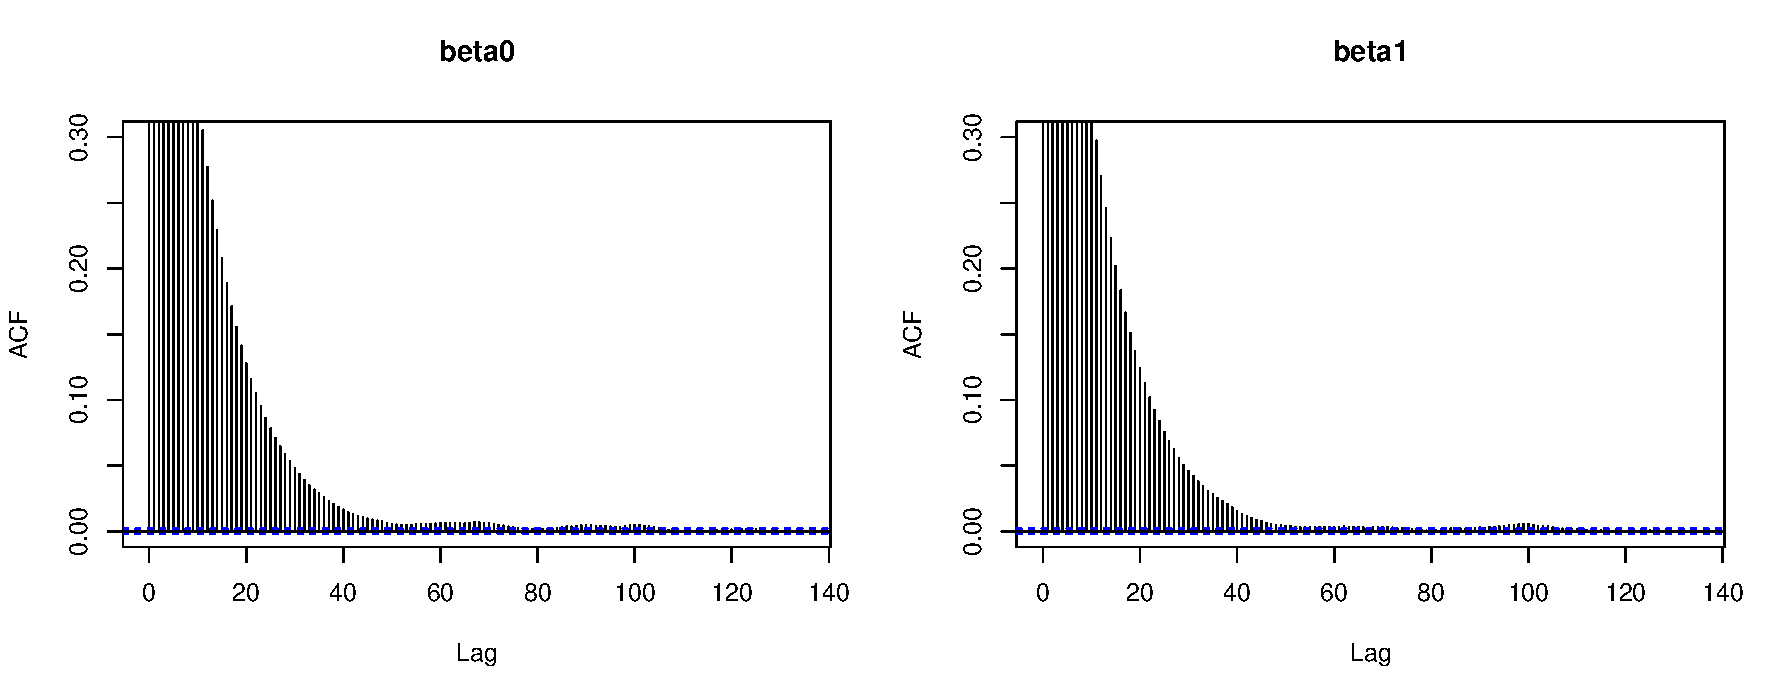
\includegraphics[width=6.0in]{acfs}
\end{figure}
\FloatBarrier
\vspace{-0.7cm}

\subquestionwithpoints{1} At what spacing should we thin the sample chains? \inred{80}

\pagebreak

Below is the histograms of MCM samples for the parameter $\beta_1$ after properly burning and thinning the chain. The vertical line is the average of the chain's values.

\vspace{-0.2cm}
\begin{figure}[htp]
\centering
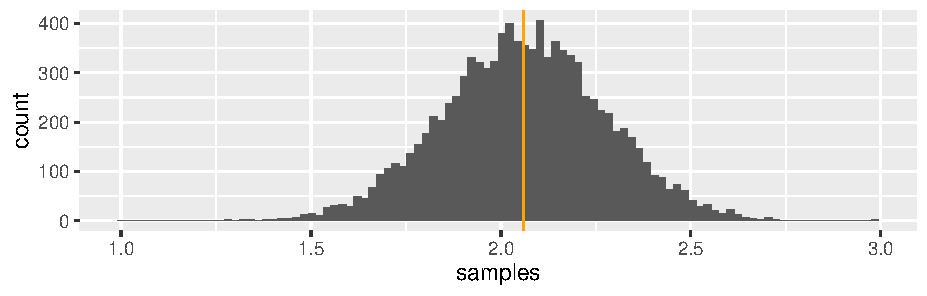
\includegraphics[width=6.0in]{beta1samples}
\end{figure}
\FloatBarrier
\vspace{-0.7cm}

\subquestionwithpoints{5} Write a detailed sentence that interprets the value of $\doublehat{\beta}_1^{MMSE}$. 

\inred{
When comparing two observations A and B sampled in the same fashion as the observations in the historical dataset were sampled, when A has $x$ 1cm larger than (B)’s $x$, then (A) is predicted to have an estimated mean count $2.05 \pm 0.25$ larger than (B)’s assuming the mean is linear in the p covariates.
}\spc{2}

\end{enumerate}


\problem There are many ways to measure to invest in the S\&P500. Two popular tickers are SPY and VOO which have market caps of 500M and 1.1T respectively and have equally low expense ratios which are about 0.1\%/yr. But are these two instruments equal? We pull the last ten years of data $n = 2581$ and we are interested in the response $Y$ which is percent daily change. We choose to use the permutation test to test the difference. Let $DGP_1$ and $DGP_2$ denote the DGP's for SPY and VOO respectively. Let $y_1$ be the values for SPY and $y_2$ be the values for VOO. 

\begin{enumerate}[(a)]
\subquestionwithpoints{2} What is the null hypothesis for this permutation test?

\beqn
H_0: \inred{DGP_1 = DGP_2} \hspace{6in}
\eeqn

\subquestionwithpoints{2} During each iteration of the permutation test, how many numeric values are divided into two groups? \\

\inred{$2581 \times 2 = 5162$}

We let $\ybar_{1} - \ybar_{2}$ be the test statistic. The test statistic on the actual data is -0.00017. Over a total of $B = 100,000$ iterations, we have the following histogram of permutation test statistic values:
\pagebreak

\vspace{-0.2cm}
\begin{figure}[htp]
\centering
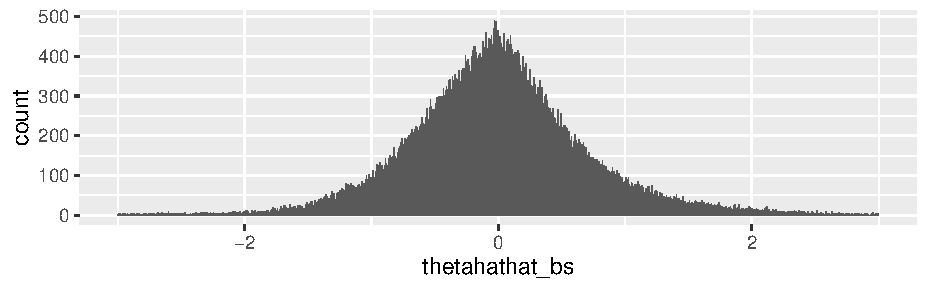
\includegraphics[width=6.0in]{perms}
\end{figure}
\FloatBarrier
\vspace{-0.7cm}

\subquestionwithpoints{1} Our choice of $B = 100,000$ is appropriate. Circle one: \inred{\fbox{yes}} / no \spc{-0.5}

\subquestionwithpoints{1} The result of this test is... Circle one: \inred{\fbox{$H_0$ retained}} / $H_0$ rejected \spc{-0.5}

\subquestionwithpoints{3} Estimate a p-value for this test. \\

\inred{$0.999$}

Now that we are reasonably convinced there's no difference between SPY and VOO, we turn to another question. We are interested in large quantiles of the percentage change. Let $\theta := \text{Quantile}[Y, 97.5\%]$. We wish to create a confidence interval for this parameter.

\subquestionwithpoints{1} Which statistical method / procedure provides asymptotically valid inference for $\theta$? The answer should be one or two words only. \\

\inred{bootstrap}

Assuming the correct answer to the previous question, we run this method and produce $B = 100,000$ iterations which we display below. 

\vspace{-0.2cm}
\begin{figure}[htp]
\centering
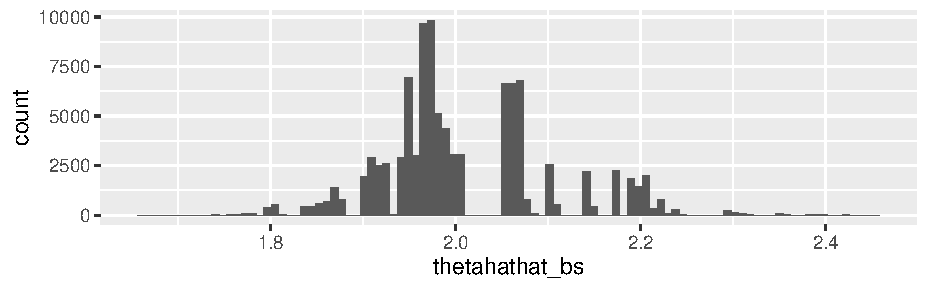
\includegraphics[width=6.0in]{bootstraps}
\end{figure}
\FloatBarrier
\vspace{-0.7cm}

\subquestionwithpoints{3} Create an approximate 95\% CI for $\theta$.  \\

\inred{$\bracks{1.85, 2.20}$}

\pagebreak
\end{enumerate}

\problem Consider $\X$ to be the the design matrix of for $n = 30$ observations and $p_{raw} = 5$ numeric covariates and their interactions. Let $\H$ be its orthogonal projection matrix. We assume also a continuous (real-valued) response model which is linear in these measurements,

\vspace{-0.2cm}
\beqn
\Y = \X\bbeta + \berrorrv.
\eeqn

\noindent For the error term, we assume the \qu{core assumption},

\vspace{-0.2cm}
\beqn
\berrorrv \sim \multnormnot{n}{\zerovec_n}{\sigsq \I_n}.
\eeqn

\noindent And the estimator for $\bbeta$ is
\beqn
\B := \XtXinvXt \Y 
\eeqn

\begin{enumerate}[(a)]
\subquestionwithpoints{4} Find the distribution of $\bv{E}$, the vector of residuals. Show each step.

\inred{
\beqn
\bv{E} &=& (\I_n - \H)\Y = (\I_n - \H)(\X\bbeta + \berrorrv) = \X\bbeta - \X\bbeta+ (\I_n - \H)\berrorrv =  \\
(\I_n - \H)\berrorrv &\sim& \multnormnot{n}{(\I_n - \H)\zerovec_n}{\sigsq (\I_n - \H)\I_n(\I_n - \H)^\top} = \multnormnot{n}{\zerovec_n}{\sigsq (\I_n - \H)}
\eeqn
}

We do not assume any structural equation model nor DAG for this phenomenon and observed measurements. We estimate $\b$ below along with selected inference information:

\begin{Verbatim}
              Estimate Std. Error t value Pr(>|t|)    
(Intercept)  9.656e+03  8.133e+03   1.187   0.2351    
x_1         -1.034e+02  1.296e+02  -0.798   0.4251    
x_2          2.322e+02  1.435e+02   1.619   0.1055    
x_3          7.178e+03  3.477e+03   2.065   0.0390 *  
x_4         -2.545e+04  3.573e+03  -7.123 1.07e-12 ***
x_5          1.983e+04  2.130e+03   9.310  < 2e-16 ***
x_1:x_2     -8.971e-01  2.306e+00  -0.389   0.6973    
x_1:x_3      6.117e+00  4.022e+01   0.152   0.8791    
x_1:x_4      3.227e+02  3.831e+01   8.423  < 2e-16 ***
x_1:x_5     -4.884e+02  2.005e+01 -24.356  < 2e-16 ***
x_2:x_3     -2.623e+02  2.771e+01  -9.465  < 2e-16 ***
x_2:x_4      8.294e+01  3.223e+01   2.573   0.0101 *  
x_2:x_5      2.294e+02  3.071e+01   7.469 8.19e-14 ***
x_3:x_4      1.069e+03  2.968e+01  36.023  < 2e-16 ***
x_3:x_5      4.614e+02  3.787e+01  12.186  < 2e-16 ***
x_4:x_5     -8.674e+02  3.807e+01 -22.784  < 2e-16 ***

Residual standard error: 1450.0
Multiple R-squared:  0.87
\end{Verbatim}
\pagebreak

Below are values of the 97.5\%iles of the Student's $T$ distribution (q) for many different degrees of freedom (df)

\begin{Verbatim}[fontsize=\footnotesize]
df      5    6    7    8    9   10  11   12   13   14   15   16   17  18   19   20
q    2.57 2.45 2.36 2.31 2.26 2.23 2.2 2.18 2.16 2.14 2.13 2.12 2.11 2.1 2.09 2.09
\end{Verbatim}

\subquestionwithpoints{4} Create a 95\% CI for $\beta$  the linear parameter for the interaction of $x_1 \times x_3$. 

\inred{
\beqn
CI_{\beta, 1- \alpha} &=& \bracks{b \pm t_{n - (p+1), 1 - \alpha/2} s_{b}} = \bracks{b \pm t_{14, .975} s_{b}} = \bracks{6.117 \pm t_{14, .975} \cdot 40.22}\\
&=& \bracks{6.117 \pm 2.14 \cdot 40.22} = \bracks{-79.95, 92.19}
\eeqn}
\vspace{-0.5cm}

\subquestionwithpoints{4} [E.C.] Consider a new observation $\x_\star = \bracks{1 ~ 1 ~ 0 ~ 0 ~ 0}$.  Create a 95\% CI for $Y_\star$. Substitute all known quantities and use the notation in the problem header for all unknown quantitites. \spc{3}

\subquestionwithpoints{2} Circle one: \inred{\fbox{$R^2_{adj} < 0.87$}} / $R^2_{adj} = 0.87$ / $R^2_{adj} > 0.87$\spc{-0.5}
\subquestionwithpoints{3} Compute the value of the $\doublehat{F}$ statistic.

\inred{
\beqn
\doublehat{F}^{-1} = \frac{p}{n-(p+1)} \parens{\oneover{R^2} - 1} = \frac{15}{14} \parens{\oneover{0.87} - 1} = 0.16 \mathimplies \doublehat{F} = 6.25
\eeqn}
\vspace{-0.5cm}


\subquestionwithpoints{2} Assume we now run the omnibus F test based on your computation in the previous question and we reject $H_0$. Also assume we did \emph{not} make a Type I error. What can you now conclude about the vector $\bbeta$? Make a numeric statement below. Hint: the answer is only a few characters. \inred{$\bbeta \neq \zerovec_{16}$}

\subquestionwithpoints{5} The regression above shows $b_1 = -103.4$ and $s_{b_1} = 129.6$.  Write the standard interpretation of $b_1$. Let the units of $x_1$ be centimeters (cm) and the units of $y$ be kilograms (kg). Underline the words in this interpretation that \emph{we know to be impossible given this specific regression}.

\inred{
When comparing two observations A and B sampled in the same fashion as the observations in the historical dataset were sampled, when A has $x_1$ 1cm larger than (B)’s $x_1$ value \underline{and otherwise shares the same measurement values}, then (A) is predicted to have an estimated response $103.4 \pm 129.6$ kg lower than (B)’s assuming the mean is linear in the p covariates.\\~\\
(The above is underlined since in a model that has interactions with the variable $x_1$, you cannot keep the value of $x_1 \times x_j$ constant for $j \neq 1$ when changing $x_1$).
}

\pagebreak
Consider instead of using the estimator $\B$ above, we use the following estimator:

\beqn
\B_{lasso} = \argmin_{\w \in \reals^{p+1}}\braces{(\Y - \X\w)^\top (\Y - \X\w) + \lambda \sum_{j=1}^{p+1}|w_j|} ~~\text{where}~~ \lambda>0
\eeqn

\subquestionwithpoints{5} Using this new estimator, circle all the quantities below that are random:

\beqn
\Aboxed{\inred{\X\quad\quad
\Y\quad\quad
\bv{E}\quad\quad
\berrorrv\quad\quad
\B\quad\quad
\B_{lasso}}}\quad\quad
\H\quad\quad
\bbeta\quad\quad
\sigsq\quad\quad
\lambda\quad\quad
n\quad\quad
p\quad
\Aboxed{\inred{s_e\quad\quad
R^2}}\quad\quad
\eeqn

\subquestionwithpoints{3} Using $\B_{lasso}$, what is the most precise numerical statement you can say about $r$, the count of the number of rejections of $H_0: \beta_j = 0$ where $j \geq 1$ at significance level $\alpha = 5\%$? \\

\inred{$r \leq 11$}

\end{enumerate}



\problem Consider the lung dataset where missingness is dropped. Survival is measured in years. Below is the code to load the data and properly code it. % and print out the first 100 survival times:

\begin{Verbatim}
> lung = na.omit(survival::lung)
> lung$status = lung$status - 1 #needs to be 0=alive, 1=dead
> surv_obj = Surv(lung$time, lung$status)
\end{Verbatim}

%> head(surv_obj,100)
%  [1]  455   210  1022+  310   361   218   166   170   567   613   707    61 
% [13]  301    81   371   520   574   118   390    12   473    26   107    53 
% [25]  814   965+   93   731   460   153   433   583    95   303   519   643 
% [37]  765    53   246   689     5   687   345   444   223    60   163    65 
% [49]  821+  428   230   840+  305    11   226   426   705   363   176   791 
% [61]   95   196+  167   806+  284   641   147   740+  163   655    88   245 
% [73]   30   477   559+  450   156   529+  429   351    15   181   283    13 
% [85]  212   524   288   363   199   550    54   558   207    92    60   551+
% [97]  293   353   267   511+
%\subquestionwithpoints{2} Some of these quantities have a \qu{+} sign appended to them. What does this indicate? \spc{2}

\noindent This dataset came with measurements for each subject. We attempt to model survival using these features using the Weibull model employing log-linear link function we discussed in class. \texttt{Age} is measured in years and \texttt{meal.cal} is measured in cal/d.  Below is the output with inference that employs the MLE core theorem:

\begin{Verbatim}
survreg(formula = surv_obj ~ age + sex + meal.cal, data = lung)

                Value Std. Error     z      p
(Intercept)  6.16e+00   6.50e-01  9.48 <2e-16
age         -1.05e-02   8.24e-03 -1.28  0.202
sex=Female   3.44e-01   1.49e-01  2.30  0.021
meal.cal     8.54e-05   1.82e-04  0.47  0.639
Log(scale)  -3.00e-01   7.29e-02 -4.11  4e-05

Scale= 0.741 
\end{Verbatim}


\begin{enumerate}

\subquestionwithpoints{4} Write an expression that estimates survival (in yr) for a 45yo male who eats 2000cal/d. Do not compute its value. 

\inred{
\beqn
\hat{y} =  e^{\x_\star\b} ~\Gamma\parens{1 + \oneover{\doublehat{k}}} = e^{6.16 + 0.00105 (45) + 0.0000854 (2000)} ~\Gamma\parens{1 + \oneover{0.741}}
\eeqn
}

\pagebreak
\subquestionwithpoints{4} [E.C.] Evaluate if this Weibull model satisfies the proportional hazard assumption.\spc{5}



Below is the output from a cox proportional hazard model with inference that employs the MLE core theorem:

\begin{Verbatim}
coxph(formula = surv_obj ~ age + sex + meal.cal, data = lung)

                  coef  exp(coef)  se(coef)       z  Pr(>|z|)  
age          0.0160863  1.0162163  0.0111394  1.444    0.149  
sex=Female  -0.4614061  0.6303966  0.1998968 -2.308    0.021 *
meal.cal    -0.0001175  0.9998825  0.0002485 -0.473    0.636 
\end{Verbatim}


\subquestionwithpoints{2} Will the above model allow you to estimate of the survival (in yr) for a 45yo male who eats 2000cal/d? Circle one: yes / \inred{\fbox{no}}  \spc{-.5}

\subquestionwithpoints{2} Will the above model predict that the survival (in yr) for a 45yo male who eats 2200cal/d is shorter than the survival (in yr) for a 45yo male who eats 2000cal/d? Circle one: \inred{\fbox{yes}} / no  \spc{-.5}


\subquestionwithpoints{5} Estimate how much more likely a 45yo female who eats 2000cal/d will survive the next week than a 45yo male who eats 2000cal/d (to the nearest two decimals). \\

\inred{$e^{-0.4614061} = 0.63$}
\end{enumerate}



\problem We are interested in the affect of exercise on HDL cholesterol. We survey $n=300$ people and measure their age (measured in years), exercise level (measured in average duration per day in minutes) and HDL cholesterol (measured in mg/dL). Below is a scatterplot of exercise on HDL cholesterol and a scatterplot of age on exercise:
\pagebreak

\vspace{-0.2cm}
\begin{figure}[htp]
\centering
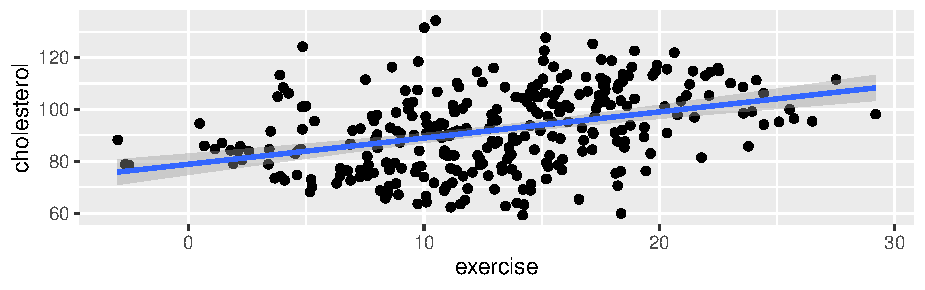
\includegraphics[width=6.0in]{exercise_cholesterol}
\end{figure}
\FloatBarrier
\vspace{-0.7cm}

\vspace{-0.2cm}
\begin{figure}[htp]
\centering
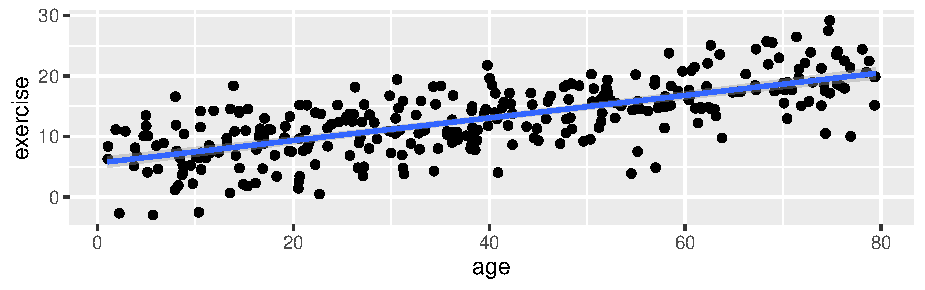
\includegraphics[width=6.0in]{age_exercise}
\end{figure}
\FloatBarrier
\vspace{-0.7cm}


\begin{enumerate}

\subquestionwithpoints{2} Is there any way to prove absolutely that the correlation between exercise and cholesterol is spurious? Circle one: yes / \inred{\fbox{no}}  \spc{-.5}
\subquestionwithpoints{1} Is there any way to prove absolutely that the correlation between age and exercise is spurious? Circle one: yes / \inred{\fbox{no}}  \spc{-.5}
\subquestionwithpoints{2} Based only on the plots above and the situation described in the problem header, is there a way to definitively assess that the regression results of the first plot is a \qu{Simpson's Paradox}? Circle one: yes / \inred{\fbox{no}}  \spc{-.5}
\subquestionwithpoints{2} Based only on the plots above and the situation described in the problem header, is there a way to definitively assess that the regression results of the first plot is a \qu{Berkson's Paradox}? Circle one: \inred{\fbox{yes}} / no  \spc{-.5}
\subquestionwithpoints{4} Draw below a DAG with nodes that include the variable names that could induce a \qu{Simpson's Paradox} bias when investigating exercise as a cause of the phenomenon HDL. 


\vspace{-0.2cm}
\begin{figure}[htp]
\centering
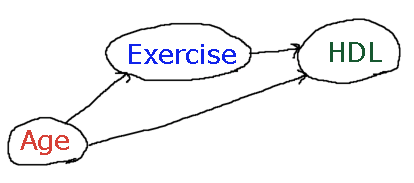
\includegraphics[width=4in]{simpsons}
\end{figure}
\FloatBarrier
\vspace{-0.7cm}

\pagebreak
\subquestionwithpoints{4} Draw below a DAG with nodes that include the variable names that could induce a partial blocking bias when investigating exercise as a cause of the phenomenon HDL. 

\vspace{-0.2cm}
\begin{figure}[htp]
\centering
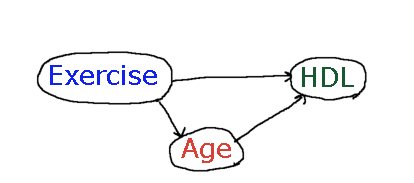
\includegraphics[width=4in]{partial_blocking}
\end{figure}
\FloatBarrier
\vspace{-0.7cm}

\end{enumerate}


\problem We are interested in understanding the effect of a pill (coded per subject as $w_i=1$) vs a placebo (coded per subject as $w_i=0$) on lowering $y$ HDL cholesterol (measured in mg/dL). We have $n=100$ subjects. We assign subjects a $w_i$ at the beginning of the study and we also record the subjects' sex, $x_i \in \braces{0,1}$, at the beginning of the study. There are 30 women and 70 men. Assume iid mean-centered noise and an additive treatment effect $\beta_T$ which we called the PATE.

\begin{enumerate}

\subquestionwithpoints{2} Is this a controlled trial? Circle one: \inred{\fbox{yes}} / no  \spc{-.5}
\subquestionwithpoints{2} Do we absolutely need to randomize the values of $w_i$ to guarantee unbiased causal inference? Circle one: yes / \inred{\fbox{no}}  \spc{-.5}
\subquestionwithpoints{2} If we use \qu{equal allocation}, what is $\sum_{i=1}^n w_i=1~\forall~\w$? \inred{50}

\subquestionwithpoints{2} Assume we proceed with an equal allocation, completely randomized design. How many possible assignments are there? \inred{$\binom{100}{50}$}
\subquestionwithpoints{3} Assume we proceed with an equal allocation, blocking design. How many possible assignments are there? \inred{$\binom{30}{15} \binom{70}{35}$}
\subquestionwithpoints{3} Assume we proceed with an pariwise matching design. How many possible assignments are there? \inred{$2^{50}$}


\subquestionwithpoints{4} Why would rerandomization be a poor choice (when compared to blocking or pairwise matching) in this scenario?\\

\inred{Rerandomization will not guarantee $x_1$ averages are equal in the pill and placebo arms. Both blocking and pairwise matching will guarantee this.}

\subquestionwithpoints{2} In order to test the sharp null, $H_0: \forall i ~y_i(w_i=1) = y_i(w_i=0)$, which procedure can you use?\\

 \inred{Fisher's Randomization Test}
\end{enumerate}


\end{document}
%%%%%%%%%%%%%%%%%%%%%%%%%%%%%%%%%%%%%%%%%%%%%%%%
%%%%%%%%%%%%%%%%%%%%%%%%%%%%%%%%%%%%%%%%%%%%%%%%

\beqn
&& \Xoneton \iid \begin{cases}
0 \withprob \theta_1 \\
1 + \poisson{\theta_2} \withprob 1 - \theta_1
\end{cases} \\
\Rightarrow && \mathcal{L}(\theta_1, \theta_2; \x) = \prod_{i=1}^n \theta_1^{\indic{x_i = 0}} \tothepow{(1 - \theta_1) \frac{\theta_2^{x_i - 1} e^{-\theta_2}}{(x_i - 1)!}}{\indic{x_i > 0}} \propto \theta_1^{n_0} (1-\theta_1)^{n - n_0} \theta_2^{\sum_{i=1}^n (x_i - 1) \indic{x_i > 0}} }  e^{-(n-n_0)\theta_2
\eeqn


\begin{enumerate}[(a)]
\subquestionwithpoints{5} Find $\cprob{\theta_1}{\theta_2, \x}$. Show that it is a brand name rv. \spc{3}

\subquestionwithpoints{5} Find $\cprob{\theta_2}{\theta_1, \x}$. Show that it is a brand name rv. \spc{3}

Using the correct answers to the first two questions, we build a Gibbs Sampler

\end{enumerate}


\problem Consider the following matrix of constant measurements:

\beqn
\X := \bracks{\onevec_n~|~\x_{\cdot 1}~|~\ldots~|~ \x_{\cdot p}}
\eeqn

\noindent with column indices $0, 1, \ldots, p$ and row indices $1, 2, \ldots, n$. We assume also a continuous (real-valued) response model which is linear in these measurements, i.e.

\beqn
\Y = \X\bbeta + \berrorrv.
\eeqn

\noindent For the error term, we assume the \qu{core assumption},

\beqn
\berrorrv \sim \multnormnot{n}{\zerovec_n}{\sigsq \I_n}.
\eeqn

\noindent And for our estimator of $\bbeta$, we choose

\beqn
\B := \XtXinvXt \Y.
\eeqn

\begin{enumerate}[(a)]

\subquestionwithpoints{5} In the \qu{linear response model assumption line} above, list the scalar parameters (if the parameter is a vector, list the scalar entries). If there are no parameters, write \qu{none}. \spc{1}

\subquestionwithpoints{5} In the \qu{core assumption} line above, list the scalar parameters (if the parameter is a vector, list the scalar entries). If there are no parameters, write \qu{none}. \spc{1}

\subquestionwithpoints{5} In the \qu{our estimator} line above, list the scalar parameters (if the parameter is a vector, list the scalar entries). If there are no parameters, write \qu{none}. \spc{1.5}

\subquestionwithpoints{10} Show that $\B$ is unbiased. \spc{6}



\noindent Now choose the following estimator instead

\beqn
\B_{\text{ridge}} := \inverse{\XtX + \lambda \I_{p+1}} \Xt \Y ~~\text{where}~\lambda > 0.
\eeqn


\subquestionwithpoints{6} Which of these two will be larger: $\normsq{\B}$ or $\normsq{\B_{\text{ridge}}}$? \spc{0.5}


\end{enumerate}


\problem This problem will analyze data from a study that investigated tooth cell growth (in length) in guinea pigs by vitamin C dose (0.5, 1 or 2mg/d) and delivery method (OJ = orange juice or VC = vitamin capsule). Here is the results of an OLS model fit to both dose and delivery method:

\begin{Verbatim}[frame=single]
                Estimate Std. Error t value Pr(>|t|)    
(Intercept)       9.2725     1.2824   7.231 1.31e-09 ***
deliveryVC       -3.7000     1.0936  -3.383   0.0013 ** 
dose              9.7636     0.8768  11.135 6.31e-16 ***
---
Signif. codes:  0 ‘***’ 0.001 ‘**’ 0.01 ‘*’ 0.05 ‘.’ 0.1 ‘ ’ 1

Residual standard error: 4.236 on 57 degrees of freedom
Multiple R-squared:  0.7038,	Adjusted R-squared:  0.6934 
F-statistic: 67.72 on 2 and 57 DF,  p-value: 8.716e-16
\end{Verbatim}

\noindent Unless otherwise noted, assume that $\berrorrv \sim \multnormnot{n}{\zerovec_n}{\sigsq \I_n}$. 
Let $\X$ denote the design matrix for this linear regression. The following quantities may be useful:

\beqn
\XtX = \bracks{\begin{array}{ccc} 60 & 30 & 70 \\ 30 & 30 & 30 \\ 70 & 35 & 105 \end{array}}, ~~~
\XtXinv = \bracks{\begin{array}{ccc} ~~0.09 & -0.03 &-0.05 \\ -0.03 &  ~~0.07 & ~~0.00 \\ -0.05 &  ~~0.00 & ~~0.04 \end{array}}, 
\eeqn

\begin{enumerate}[(a)]

\subquestionwithpoints{5} What is the sample size $n$ of this dataset?\spc{-0.5}

\subquestionwithpoints{5} Test $H_0: \beta_{\text{dose}} = 0$ at $\alpha = 5\%$. \spc{2}

\subquestionwithpoints{5} Create a 95\% CI for the effect of delivery being a vitamin capsule instead of orange juice. The t-value to use in this computation is 2.00. \spc{2}

\subquestionwithpoints{5} Run the omnibus test at $\alpha = 5\%$. \spc{1}

\subquestionwithpoints{10} For a guinea pig who was given orange juice and 1mg of vitamin C, provide a 95\% CI for the guinea pig's tooth cell growth. The t-value to use in this computation is 2.00. \spc{8}


\subquestionwithpoints{10} Assuming independence of errors and homoskedasticity of errors, test $H_0: \beta_{\text{dose}} = 10$ at $\alpha = 5\%$. \spc{4}


\subquestionwithpoints{5} Is there enough information here to test $H_0: \beta_{\text{dose}} = 0$ at $\alpha = 5\%$ if we assume independent, mean-centered and heteroskedastic errors? Yes / No \spc{-0.5}

In reality, we are unsure of the distribution of the errors but we know that due to the way the data was sampled, we are guaranteed that the errors are independent. Hence use a bootstrap. We are interested in inference for the effect of delibery being a vitamin capsule instead of orange juice. The top of the following page shows the result of 1,000 boostrap samples where each time, the OLS for this effect was computed. The vertical lines indicate the empirical 2.5\%ile and 97.5\%ile.


\begin{figure}[htp]
\centering
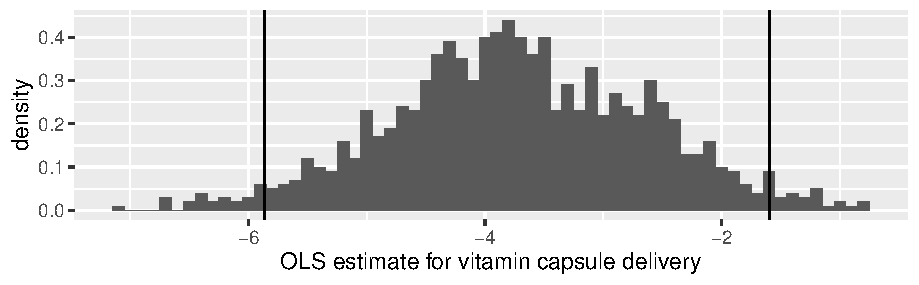
\includegraphics[width=6.5in]{bootstrap}
\end{figure}
\FloatBarrier


\subquestionwithpoints{5} Using the boostrap samples, test $H_0: \beta$ for vitamin capsule delivery is zero at $\alpha = 5\%$. \spc{2}


\end{enumerate}

\problem This problem will analyze data from a study that investigated the number of yarn breaks by two features: type of yarn wool (A or B) and amount of tension (L = low, M = medium, H = high). Since the response being modeled is a count, we choose a negative binomial model which is more flexible than a Poission model. We parameterize the negative binomial with parameters $r, \theta$ where its expectation is $\theta$. We link $\theta$ to the two features using the link $\theta_i = e^{\x_i \bbeta}$ for $i = 1, \ldots, n$. Below is the summary for the inference of $\bbeta$ for both features (the inference for $r$ is omitted). We also display the log-likelihood of this model.

\begin{Verbatim}[frame=single]
            Estimate Std. Error z value Pr(>|z|)    
(Intercept)   3.6734     0.0979  37.520  < 2e-16 ***
woolB        -0.1862     0.1010  -1.844   0.0651 .  
tensionM     -0.2992     0.1217  -2.458   0.0140 *  
tensionH     -0.5114     0.1237  -4.133 3.58e-05 ***

'log Lik.' -199.3819 (df=5)
\end{Verbatim}

\noindent Here are outputs for two other models:

\begin{Verbatim}[frame=single]
            Estimate Std. Error z value Pr(>|z|)    
(Intercept)  3.43518    0.08071  42.562   <2e-16 ***
woolB       -0.20599    0.11533  -1.786   0.0741 .  

'log Lik.' -206.9874 (df=3)
\end{Verbatim}

\begin{Verbatim}[frame=single]
            Estimate Std. Error z value Pr(>|z|)    
(Intercept)  3.59426    0.08715  41.243  < 2e-16 ***
tensionM    -0.32132    0.12557  -2.559   0.0105 *  
tensionH    -0.51849    0.12739  -4.070  4.7e-05 *** 

'log Lik.' -201.0109 (df=4)
\end{Verbatim}

\noindent Here are some values of the inverse CDF of the $\chisq{df}$ distribution:

\begin{Verbatim}[frame=single,fontsize=\footnotesize]
                Probability less than the critical value
  df          0.90      0.95     0.975      0.99     0.999
----------------------------------------------------------
  1          2.706     3.841     5.024     6.635    10.828
  2          4.605     5.991     7.378     9.210    13.816
  3          6.251     7.815     9.348    11.345    16.266
  4          7.779     9.488    11.143    13.277    18.467
  5          9.236    11.070    12.833    15.086    20.515
  6         10.645    12.592    14.449    16.812    22.458
  7         12.017    14.067    16.013    18.475    24.322
\end{Verbatim}

\begin{enumerate}[(a)]

\subquestionwithpoints{4} Is the parameter $r$ a nuisance parameter? Yes / No \spc{-0.5}

\subquestionwithpoints{6} Calculate the likelihood ratio test statistic for the test that tension has no effect on number of yarn breaks. \spc{1.5}

\subquestionwithpoints{3} Test the null hypothesis that tension has no effect on number of yarn breaks at $\alpha=5\%$. Justify your answer. \spc{2}

\subquestionwithpoints{6} The maximum likelihood estimate of $r$ is 9.94. Given a piece of yarn with wool type B and low tension, predict the number of yarn breaks it will have to the nearest number of yarn breaks. \spc{2}


\end{enumerate}
\end{document}

